% pooling, kernel (3,3), stride (2,2)
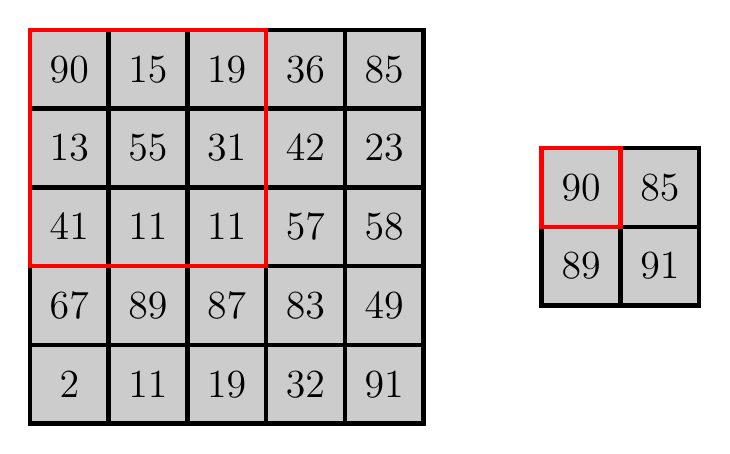
\begin{tikzpicture}
    \coordinate (p) at (0,0);
    \draw[
        ultra thick,
        step=1, 
        color=black,
        draw=black,
        fill=black!20!white,
        shift={(p)}
    ] (0,0) grid (5,-5) rectangle (0,0)
    foreach[count=~] \l in {90, 15, 19, 36, 85, 13, 55, 31, 42, 23, 41, 11, 11, 57, 58, 67, 89, 87, 83, 49,  2, 11, 19, 32, 91} {
        ({0.5+mod(~-1,5}, {-0.5-div(~-1,5}) node {\Large \l}
    };
    \draw[shift={(p)}, draw=red, ultra thick] (0,0) rectangle (3,-3);
    
    \coordinate (p) at (6.5,-1.5);
    \draw[
        ultra thick,
        step=1, 
        color=black,
        draw=black,
        fill=black!20!white,
        shift={(p)}
    ] (0,0) grid (2,-2) rectangle (0,0)
    foreach[count=~] \l in {90, 85, 89, 91} {
        ({0.5+mod(~-1,2}, {-0.5-div(~-1,2}) node {\Large \l}
    };
    \draw[shift={(p)}, draw=red, ultra thick] (0,0) rectangle (1,-1);
    % max     {90, 85, 89, 91}
    % average {32, 40, 38, 54}
\end{tikzpicture}
